\section{Data Model}
\label{sec:dataModel}

In this section, provide details of your dimensions, why they are in your data model, how sources of data contribute to each of the dimensions, and present your star schema. 

Do not do this:

\begin{figure}[ht]
\centering
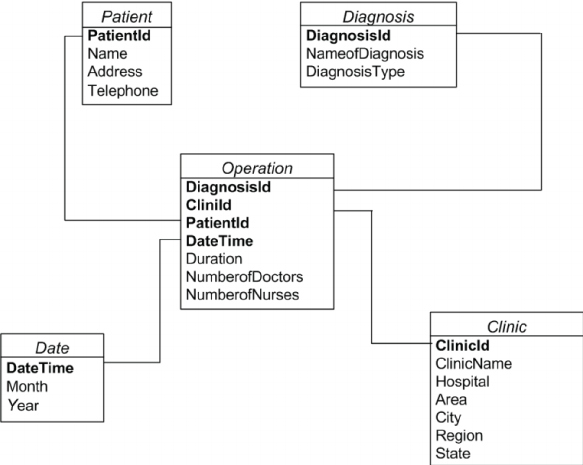
\includegraphics[width=.6\textwidth]{figures/sampleStar.png}
\caption{Some star schema i found online}
\label{fig:star}
\end{figure}

So i have 4 dimensions, as seen in \figurename~\ref{fig:star}. They are good and answer all the queries. I was lazy, so i took a screen shot of SSAS, which my lecturer cannot read.

Instead, provide a detailed discussion on the composition of each dimension, justifying its contents and any hierarchies you have designed in to facilitate drill down. It's seriously unlikely that you can map a dataset 1 to 1 with all columns to a dimension, so explain here which components of which dataset map to which dimension. For the fact table, be precise with respect to the granularity of the facts, and motivate each fact included linking it to at least one of your requirements.